% Author: Keshav (condensed from report/section_classical_baseline.md)
\section{Classical baseline: LightGBM on pair features}
\label{sec:classical}

The classical matcher is a gradient-boosted tree classifier, LightGBM, on 48
hand-built features of each candidate pair (S2/S3 record $q$, S1 candidate $s$), in six families:
\begin{itemize}
  \item \textbf{name strings} (14): edit-distance similarities of the normalised names (Indel ratio,
        token-set / token-sort / partial ratio, Jaro--Winkler, word Jaccard), the same on the name without
        its legal form, words found in only one name, and conflicting legal forms;
  \item \textbf{address strings} (6): the same similarities on the address;
  \item \textbf{numbers} (4): digit strings in the two addresses (house, plot or shop numbers): Jaccard,
        count found only in $q$ or only in $s$, first number equal;
  \item \textbf{parsed fields} (7): field-by-field comparison of the BiLSTM-CRF parses (Section~\ref{sec:parsing});
  \item \textbf{retrieval} (8): \nb{03}'s TF-IDF and fine-tuned e5 cosines, their ranks, the RRF rank;
  \item \textbf{metadata} (9): script and source of $q$, empty address, text lengths.
\end{itemize}
Gap and rank features compare a candidate with the \emph{other candidates of the same record}, since the
decision is relative: does this S1 beat the other four? The model is trained on the 1.51M part-A pairs with
early stopping on val log-loss and reaches 1,609 trees in 4.6 minutes on a CPU.

\paragraph{Results.} The GBM reaches \textbf{0.9908} test \fhalf{} (P 0.9938, R 0.9873). It is the third-best
single model, 0.0004 behind the fully fine-tuned 278M-parameter bge cross-encoder (Table~\ref{tab:main}),
and its singleton accuracy (0.9857) is second only to mDeBERTa-v3.

\begin{figure}[h]
\centering
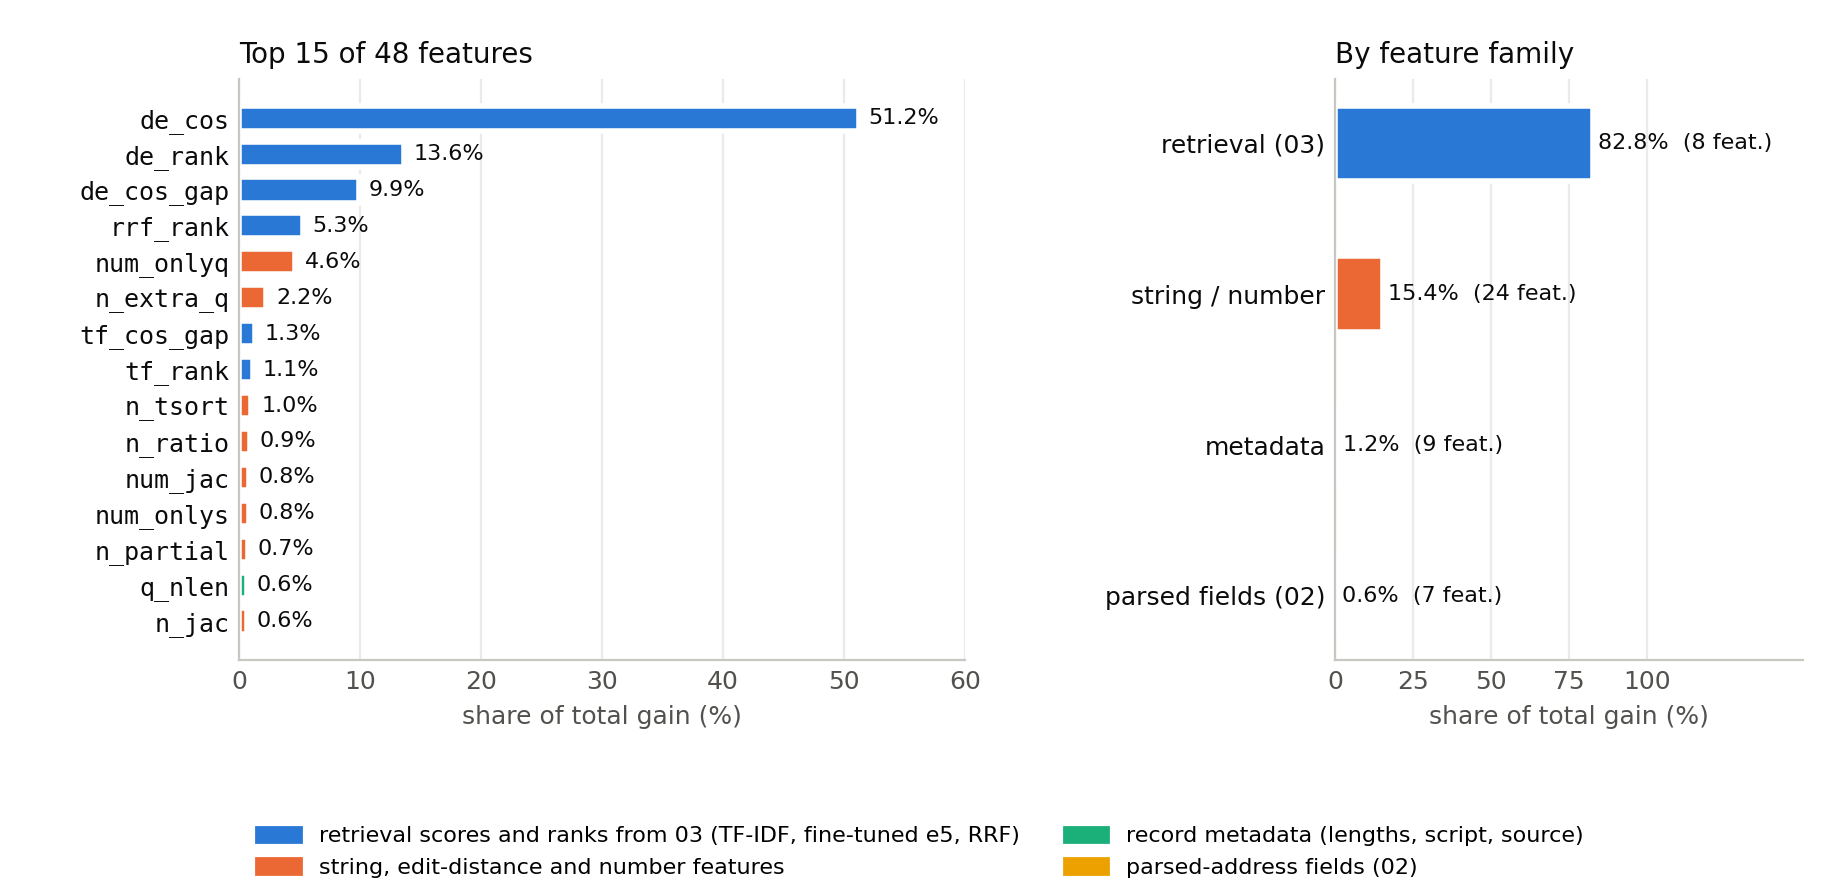
\includegraphics[width=0.92\linewidth]{gbm_feature_gain.png}
\caption{Share of the LightGBM split gain per feature (left, top 15 of 48) and per family (right).}
\label{fig:gbmgain}
\end{figure}

\paragraph{What the model uses.} Figure~\ref{fig:gbmgain} shows that \textbf{83\% of the gain comes from
\nb{03}'s retrieval features}. The fine-tuned e5 cosine alone has 51.2\%: it was trained on this task, and it
reads the original-script name, so it already captures matches that string ratios miss. Its rank (13.6\%)
and its gap to the best candidate (9.9\%) follow. The strongest hand-built feature is \texttt{num\_onlyq}
(4.6\%), the count of numbers in $q$'s address that do not appear in $s$. It is a hard negative signal: two
branches of a chain have near-identical names but different street numbers, and the embeddings blur exactly
that difference. String and number features together have 15.4\% of the gain (numbers 6.5\%), metadata
1.2\% and the parsed fields 0.6\%. So the GBM is a classical learner \emph{on top of a neural retriever}, not
a pure edit-distance model. We did not run it without the retrieval features.

\paragraph{Does the parser help matching?} We ran the GBM twice, once with BiLSTM-CRF fields and once with
rule fields. Test \fhalf{} is 0.99081 vs.\ 0.99051. A paired bootstrap over the 21,529 test
entities (10,000 resamples) gives a 95\% interval for the difference of
$[-0.00006, +0.00064]$. It includes 0, so the difference is \textbf{not significant}. The runs differ on only
273 entities (137 better with the BiLSTM-CRF, 136 with the rules). This is expected: with commas, both
parsers give the same fields for 99.7\% of addresses, and the parsed fields carry little gain. The parser's
advantage, comma-free addresses, does not occur in this data.
